\chapter{Wissenschaftliche Grundlagen} \chaplabel{grundlagen}

In diesem Kapitel werden die für das maschinelle Lernen im Rahmen unseres Projektes relevanten Grundlagen erläutert.

\section{Maschinelles Lernen}

Lernen ist, nach \citet[\citechap{7}]{poole-artificial-intelligence}, die Fähigkeit eines Agenten anhand von Erfahrungen das eigene Verhalten zu verbessern. Hierbei wird sowohl die Genauigkeit als auch die Geschwindigkeit bei der Bearbeitung von Aufgaben verbessert und die Bandbreite der gezeigten Verhaltensmuster erweitert.

Es existieren zahlreiche Methoden des maschinellen Lernens. Diese können in verschiedene Kategorien eingeteilt werden, ich werde hier auf überwachtes und unüberwachtes Lernen~\cite{web:supunsup} eingehen.

Beim überwachten Lernen werden dem Lernalgorithmus sowohl die Eingabedaten, als auch deren Zielwerte zur Verfügung gestellt. Der Algorithmus soll nun die Abbildungsfunktion
$$f: \text{Eingabedaten} \mapsto \text{Zielwerte}$$
erlernen, er versucht anhand der Eingabedaten die Zielwerte zu ermitteln. Zunächst macht der Algorithmus dabei noch Fehler. Anhand der bereitgestellten Zielwerte kann der Fehler ermittelt und das Verhalten angepasst werden, um in der Zukunft bessere Vorhersagen machen zu können. Die Fehler werden in Kosten angegeben, welche durch eine geeignete Kostenfunktion errechnet werden. Diese Kosten gilt es zu minimieren.

Um das Gelernte zu überprüfen, folgt auf eine Trainingsphase mit den zugehörigen Zielwerten eine Testphase ohne Zielwerte. Der Algorithmus muss das vorher Gelernte in der Testphase auf unbekannte Daten anwenden. Die Verwendung eines anderen Datensatzes ist sehr wichtig, da die Gefahr besteht, dass sich der Algorithmus zu sehr auf die Lerndaten einstellt und dadurch die Generalisierungsfähigkeit verliert.

\begin{figure}
    \centering
    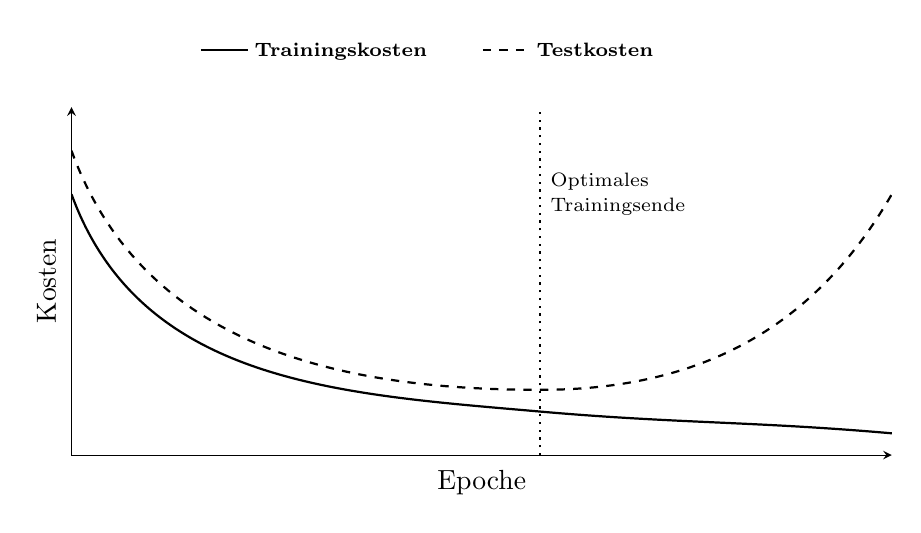
\begin{tikzpicture}[
    curve/.style={
        thick,
        domain=0:14,
    },
]

    \begin{axis}[
        width=12cm,
        height=6cm,
        axis x line=center,
        axis y line=center,
        xmin=0, xmax=14,
        ymin=0, ymax=8,
        xlabel=Epoche, xtick style={draw=none}, xtick=\empty,
        ylabel=Kosten, ytick style={draw=none}, ytick=\empty,
        xlabel near ticks,
        ylabel near ticks,
        legend columns=-1,
        legend style={
            at={(0.5,1.1)},
            anchor=south,
            draw=none,
            font=\scriptsize\bfseries,
            text width=8em,
            text height=1.5ex,
            text depth=.5ex,
        },
    ]
        \draw[curve]
            (axis cs:0,6) to[out=-70,in=175]
            (axis cs:8,1) to[out=-5,in=175]
            (axis cs:14,0.5);

        \draw[curve, dashed]
            (axis cs:0,7) to[out=-70,in=180]
            (axis cs:8,1.5) to[out=0,in=240]
            (axis cs:14,6);

        \addlegendimage{curve}
        \addlegendentry{Trainingskosten}
        \addlegendimage{curve,dashed}
        \addlegendentry{Testkosten}

        \draw[dotted, thick] (axis cs:8,0) -- node[near end,right,text width=5em]{\scriptsize{Optimales\\[-1ex]Trainingsende}} (axis cs:8,8);
    \end{axis}
\end{tikzpicture}

    \caption[Overfitting]{Overfitting. Die Trainings- und Testkosten nehmen zunächst beide ab, dann steigen die Testkosten wieder, während die Trainingskosten weiterhin optimiert werden. Dies ist der Zeitpunkt, ab dem der Algorithmus seine Generalisierungsfähigkeit verliert.}
    \figlabel{fig:overfitting}
\end{figure}

Dieses Phänomen wird auch \fremdwort{Overfitting} genannt \citep{overfitting}. In \figref{fig:overfitting} sind beispielhafte Kosten der Trainings- und der Testphasen im Verlauf der Lernepochen zu sehen. Die Kostenfunktion der Trainingsdaten wird optimiert, sodass bestenfalls die Kosten bei den Testdaten ebenfalls sinken. Zunächst ist dies auch der Fall, doch ab einem gewissen Punkt sinken die Kosten bei den Trainingsdaten, die Kosten für den Testdatensatz steigen jedoch wieder an. Dies ist der Moment, in dem das Netz die Generalisierungsfähigkeit verliert und ein Overfitting beginnt. Es ist meist sinnvoll, an diesem Punkt den Lernvorgang zu beenden.

Überwachtes Lernen findet vor allem Anwendung in Klassifizierungsproblemen und in sogenannnten Regressionsproblemen, bei denen die Zielwerte numerisch, etwa Geldbeträge oder bestimmte Gewichtsmaße sind.

Im Vergleich zum überwachten Lernen werden beim unüberwachten Lernen keine Zielwerte angegeben, der Algorithmus erhält also ausschließlich die Eingabedaten. Er lernt keine Abbildungsfunktion, sondern vielmehr ein Modell der Struktur beziehungsweise die Verteilung der Eingabedaten~\cite{web:supunsup}.

Häufig werden unüberwachte Lernalgorithmen verwendet, um Daten nach bestimmten Eigenschaften zu gruppieren. Es werden dabei Gruppen gebildet, deren Elemente sich möglichst ähnlich sind. Dieser Vorgang wird auch \fremdwort{Clustering} genannt \citep[\citechap{11.1}]{poole-artificial-intelligence} .

Für unser Projekt haben wir uns für überwachtes Lernen entschieden, da wir einen gut definierten Hypothesenraum haben und zudem Trainingsdaten inklusive Zielwert recht einfach generieren können, da wir beim Tippen die Daten des Handschuhs mit den vom Computer verzeichneten Tastenanschlägen verbinden können.

Es gibt viele verschieden ML-Methoden, die überwachtes Lernen verwenden. Wir haben uns für künstliche neuronale Netze (NN) entschieden. Diese bieten eine breitgefächerte Variation an Anwendungsmöglichkeiten und sind in der Lage, komplexe Zusammenhänge in den Daten zu erkennen und für die gemachten Ausgaben zu verwenden. Wenn ein neuronales Netz gelernt ist, kann es in der Anwendung die Ausgaben sehr schnell berechnen.

Nachteile eines neuronalen Netzes sind unter anderem, dass sie eine große Menge an Lerndaten benötigen und oft sehr viel Training erfordern, um zufriedenstellende Ergebnisse zu erzielen. Zudem ist es sehr schwer, die vom Netz gelernten Zusammenhänge einzusehen. Außerdem muss darauf geachtet werden, dass kein Overfitting auftritt, neuronale Netze sind hierfür anfällig.

\section{Künstliche Neuronale Netze}

Künstliche neuronale Netze werden im Bereich des maschinellen Lernes häufig verwendet. Durch die verschiedenen Strukturen von neuronalen Netzen finden sie Anwendung in sehr unterschiedlichen Bereichen des Lernens, unter anderem in Muster- und Spracherkennung, aber auch in der Bildverarbeitung oder beim Lernen von Bewegungsabläufen.

Neuronale Netze sind an Gehirnstrukturen angelehnt, gleichen diesen jedoch nicht vollständig~\cite{web:misconceptions-neural-network}.
Grundbausteine sind einzelne Neuronen (Einheiten), welche über gewichtete Kanten miteinander verbunden sind. Diese Kanten werden mit zufälligen Werten initialisiert und nach und nach so angepasst, dass sie für die ihnen gestellte Aufgabe möglichst gut geeignet sind.

Die Struktur eines Netzes ist von großer Bedeutung und kann zwischen verschiedenen Netztypen stark variieren. Die einfachste Struktur ist wohl die des \emph{Feedforward-Netz} \citep{feedforward}. Hierbei sind verschiedene Schichten, welche unterschiedlich viele Einheiten enthalten können, hintereinandergeschaltet und mit Kanten verbunden. Das Netz ist nach vorne gerichtet, die Kanten gehen also von einer Schicht ausschließlich in die nächste, ohne Schleifen oder rückwärtsgerichtete Kanten.

Das Netz rechnet, indem die Eingabeschicht (\fremdwort{input layer}) die Eingabedaten erhält. Jede Einheit der Schicht ermittelt mit einfachen mathematischen Mitteln einen eigenen Ausgabewert. Dieser wird von den gewichteten Kanten in die nächste Schicht geleitet, bis die Ausgabeschicht (\fremdwort{output layer}) erreicht wird. Die von der Ausgabeschicht ermittelten Werte werden dann als Ergebnis interpretiert.

Es gibt viele verschieden mathematische Mittel, welche verwendet werden können. Diese sind an sich jedoch primitiv im Vergleich zur Ausdrucksstärke des Netzes. Durch die Verwendung vieler Einheiten steigt die Komplexität der Berechnungen, welche mit dem Netz durchgeführt werden können.

Die \emph{Backpropagation-Methode} wird beim überwachten Lernen eingesetzt. Dabei wird zunächst der Ausgabewert mit dem tatsächlichen Wert verglichen. Der ermittelte Fehler wird auf die Kanten verteilt, welche den Fehler verursacht haben und die Kanten werden dementsprechend angepasst. Dadurch ist das Netz in der Lage, Ausgabewerte zu generieren, die möglichst oft dem Zielwert entsprechen.

Im Folgenden werde ich auf zwei verschiedene Strukturen neuronaler Netze eingehen, welche wir in diesem Projekt nutzen.

\subsection{Recurrent Neural Network}

Zunächst haben wir mit einem einfachen \fremdwort{Recurrent Neural Network} \citep[RNN;][]{elman-rnn} gearbeitet. Ein RNN unterscheidet sich vom einfacheren Feedforward-Netz vor allem dadurch, dass es die aufeinanderfolgenden Eingabewerte nicht als unabhängig behandelt, sondern eine Relation zwischen diesen herstellen kann. Das ermöglicht ein Lernen von Sequenzen.

Die Struktur eines RNN ist in \figref{rnn} vereinfacht dargestellt. Nach der Eingabeschicht, in welcher die zu lernenden Daten eingespeist werden, folgt eine versteckte Schicht (\fremdwort{hidden layer}). Jede Einheit dieser Schicht ist mit jeder anderen verbunden, zuzüglich verfügen die Einheiten über Schleifen, also Kanten zu sich selbst. Dies führt dazu, dass die Informationen aus der Eingabeschicht in die versteckte übergehen, und hier beliebig lange verweilen, bevor sie zur Ausgabeschicht (oder gegebenenfalls zu weiteren Zwischenschichten) weitergereicht werden. Das Netz kann sich dadurch Informationen aus den vorherigen Eingaben merken und für die Berechnung nachfolgender Ausgaben verwenden.

\begin{figure}
    \centering
    \begin{tikzpicture}[
    ->,
    >=stealth',
    shorten >=1pt,
    auto,
    node distance=2.2cm,
    semithick,
    layer/.style={
        draw,
        minimum width=0.9cm,
        minimum height=6cm,
    },
    bend angle=15,
    every state/.style={
        very thick,
        fill=white,
        distance=1.2,
        minimum size=0.5cm,
    },
]
    \node[state]         (D)  {};
    \node[state]         (A) [above left=1cm and 2.2cm of D] {};
    \node[state]         (B) [below left=1cm and  2.2cm of D] {};

    \node[state]         (C) [above of=D] {};

    \node[state]         (E) [below of=D] {};
    \node[state]         (F) [right =2.2cm of D] {};

    \path   (A) edge              node {} (C)
                edge              node {} (D)
                edge              node {} (E)

              (B) edge              node {} (C)
                edge              node {} (D)
                edge              node {} (E)

            (C) edge [loop above,gray] node {} (C)
                edge              node {} (F)
                edge [bend left,gray]  node {} (D)
                edge [bend left,gray]  node {} (E)

            (D) edge [loop above,gray] node {} (D)
                edge              node {} (F)
                edge [bend left,gray]  node {} (C)
                edge [bend left,gray]  node {} (E)

            (E) edge [loop above,gray] node {} (E)
                edge [bend left,gray]  node {} (C)
                edge [bend left,gray]  node {} (D)
                edge              node {} (F);


    \node[layer,label=below:{\small\textbf{input}}] at ($(A) !.5! (B)$) {};
    \node[layer,label=below:{\small\textbf{hidden}}] at (D) {};
    \node[layer,label=below:{\small\textbf{output}}] at (F) {};
    % \draw ($(E.south west) - (0.2, 0.2)$) rectangle ($(C.north east) + (0.2, 0.2)$);
    % \draw ($(F.south west) - (0.2, 0.2)$) rectangle ($(F.north east) + (0.2, 0.2)$);

\end{tikzpicture}

    \caption[Struktur eines RNN]{Struktur eines RNN, bestehend aus einer Eingabeschicht, einer versteckten Schicht und einer Ausgabeschicht.}
    \figlabel{rnn}
\end{figure}

\subsection{Convolutional Network}

Eine weitere Art des neuronalen Netzes ist das sogenannte \fremdwort{Convolutional Neural Network} \citep[CNN, manchmal übersetzt als ,,Faltungsnetz'';][]{cnn_orig}.  Mithilfe von Merkmalserkennung
 % (engl. \fremdwort{Feature detection})
werden prägnante Teile eines Datensatzes ermittelt, um diesen dann zu klassifizieren.

Durch das Extrahieren von Merkmalen sind CNNs außerordentlich gut darin, Muster zu erkennen. Sie finden dementsprechend oft Anwendung in der Textverarbeitung sowie in der Sprach-, Bild- und Handschriftserkennung \citep{sentence_classification, speech_recognition}.

\begin{figure}
    \centering
    \begin{tikzpicture}
    \matrix(start)[
        matrix of nodes,
        inner sep=0pt,
        draw,
        nodes={
            inner sep=0pt,
            text width=.5cm,
            align=center,
            minimum height=.5cm,
            draw,
        }
    ]{
       5  & 2 & 3 & 8 \\    0 & |[fill=primary!25]|{1} & 2 & 6 \\    4 & 8 & 5 & 4 \\    1 & 7 & 1 & 7\\};

    \matrix(filter0)[
        inner sep=0pt,
        draw,
        label=above:{\tiny{}Filter 0},
        opacity=0.5,
        above right=-0.2cm and 0.8cm of start,
        matrix of nodes,
        nodes={
            inner sep=0pt,
            text width=.5cm,
            align=center,
            minimum height=.5cm,
            draw,
        },
    ]{
        0 & 1 & 0 \\    0 & 1 & 0 \\    0 & 1 & 0 \\};
    \matrix(filterN)[
        inner sep=0pt,
        draw,
        label=above:{\tiny{}Filter N},
        opacity=0.5,
        below right=-0.2cm and 0.8cm of start,
        matrix of nodes,
        nodes={
            inner sep=0pt,
            text width=.5cm,
            align=center,
            minimum height=.5cm,
            draw,
        },
    ]{
        0 & 0 & 1 \\    0 & 1 & 0 \\    1 & 0 & 0 \\};

    \node (rect) at (-0.25, 0.25) [draw=primary,line width=0.6mm,minimum width=1.5cm,minimum height=1.5cm] {};
    \draw[->, thick, primary] (rect) -- (filter0);
    \draw[->, thick, primary] (rect) -- (filterN);

    \matrix(conv0)[
        matrix of nodes,
        inner sep=0pt,
        draw,
        right=of filter0,
        label=above:{\tiny{Feature Map 0}},
        nodes={
            inner sep=0pt,
            text width=.5cm,
            align=center,
            minimum height=.5cm,
            draw,
        }
    ]{
        5 & 3 & 5 & 14 \\    9 & |[fill=primary!25]|{11} & 10 & 18 \\    5 & 16 & 8 & 17 \\    5 & 15 & 6 & 11\\};

    \matrix(convN)[
        matrix of nodes,
        inner sep=0pt,
        draw,
        right=of filterN,
        label=above:{\tiny{}Feature Map N},
        nodes={
            inner sep=0pt,
            text width=.5cm,
            align=center,
            minimum height=.5cm,
            draw,
        }
    ]{
        5 & 2 & 4 & 10 \\    2 & |[fill=primary!25]|{8} & 18 & 11 \\    5 & 11 & 18 & 5 \\    9 & 12 & 5 & 7\\};

    \node (rect2) at ($(conv0) + (-0.5, 0.5)$) [draw=orange,line width=0.6mm,minimum width=1cm,minimum height=1cm] {};
    \node (rect2) at ($(convN) + (-0.5, 0.5)$) [draw=orange,line width=0.6mm,minimum width=1cm,minimum height=1cm] {};
    \matrix(pool0)[
        inner sep=0pt,
        draw,
        label=above:{\tiny{}Pool 0},
        right=of conv0,
        matrix of nodes,
        nodes={
            inner sep=0pt,
            text width=.5cm,
            align=center,
            minimum height=.5cm,
            draw,
        },
    ]{
        |[fill=orange!25]|{11} & 18 \\    16 & 17 \\};
    \matrix(poolN)[
        inner sep=0pt,
        draw,
        label=above:{\tiny{}Pool N},
        right=of convN,
        matrix of nodes,
        nodes={
            inner sep=0pt,
            text width=.5cm,
            align=center,
            minimum height=.5cm,
            draw,
        },
    ]{
        |[fill=orange!25]|{8} &  18\\    12 & 18 \\};
    % \draw(rect)[primary, line width=0.65mm] (-1,-0.5) rectangle (0.5,1);
    \draw[->, line width=1pt, primary,bend angle=20] (filter0.east |- conv0-2-2.north west) to[bend left] (conv0-2-2.north west);
    \draw[->, line width=1pt, primary,bend angle=20] (filterN.east |- convN-2-2.north west) to[bend left] (convN-2-2.north west);
    \draw[->, line width=1pt, orange,bend angle=20] (conv0-2-2.east |- pool0-1-2.north west) to[bend left] (pool0-1-1.north west);
    \draw[->, line width=1pt, orange,bend angle=20] (convN-2-2.east |- poolN-1-2.north west) to[bend left] (poolN-1-1.north west);
    \node[font=\Large] at ($(filter0)!0.45!(filterN)$) {$\vdots$};
    % \path   (rect) edge              node {} (filter0)
            % (rect) edge              node {} (filterN);

    \node[font=\Large] at ($(conv0)!0.45!(convN)$) {$\vdots$};
\end{tikzpicture}

    \caption[Merkmalsextraktion eines CNN]{Extrahieren von Merkmalen durch ein CNN: Anwendung der Filter und Ausführung eines Max-Poolings. Die Filter betrachten jeden Wert der Eingabedaten und ermitteln anhand der Nachbarschaftswerte und ihrer eigenen Gewichtung neue Werte, welche bestimmte Merkmale hervorheben. Das Max-Pooling wählt aus disjunkten Vierecken den maximalen Wert, um die Datenmenge zu reduzieren und besondere Merkmale hervorzuheben.}
    \figlabel{fig:cnn}
\end{figure}

\figref{fig:cnn} zeigt, wie ein CNN Merkmale aus Eingabedaten extrahiert.
Hierbei werden verschiedene Filter angewendet, um Merkmale der Daten  hervorzuheben.
Zunächst werden die Daten in die Eingabeschicht gegeben. Bei einer Bild\-erkennung wären dies zweidimensionale Werte, welche die Pixel des Bildes repräsentieren.
Es wird nun jeder Wert (in der Grafik rot unterlegt) inklusive seiner Nachbarn (rotes Viereck) mit jedem der \fremdwort{n} Filter multipliziert.
Jeder Filter ist zu Beginn mit zufälligen Werten belegt und wird über die Zeit trainiert, bis er ein bestimmtes Merkmal besonders gut hervorheben kann.

Bei der schrittweisen Multiplikation der Eingangsschicht mit den Filtern entstehen \fremdwort{n}~sogenannte \fremdwort{Feature Maps} (deutsch: Merkmalsabbildungen). In jeder Feature Map ist ein bestimmtes Merkmal der Daten hervorgehoben, abhängig vom zugehörigen Filter.
Nach der Extraktion der Merkmale wird im nächsten Schritt das sogenannte \fremdwort{Pooling} (deutsch: Bündelung) vorgenommen. Hierbei wird die Eingabematrix in disjunkte Vierecke geteilt, aus denen jeweils ein Wert entnommen wird, mit welchem weitergerechnet wird.
Es gibt unterschiedliche Methoden des Poolings. In unserem Projekt haben wir uns für das Max-Pooling entschieden, bei dem der höchste Wert aus der \num{2x2}-Matrix verwendet wird.

%Das Pooling kann durch das Verwerfen von Daten auch ein Mittel gegen Overfitting sein.\cn

Das Anwenden der Filter (\fremdwort{Convolution}-Schritt) und das Pooling werden wiederholt. Nach der letzten Iteration werden die aktuellen Feature Maps in eine oder mehrere vollständig verbundene versteckte Schichten geführt, welche die nun bereits stark angepassten und reduzierten Daten schließlich klassifizieren. Durch die vorherige Aufbereitung und Reduzierung der Daten wurde die Aufgabe des Klassifizierens stark vereinfacht, dies ist wesentlich einfacher als eine direkte Klassifikation der Eingabedaten.

Die von dem CNN ermittelte Klasse der eingegebenen Daten wird mit dem eigentlichen Zielwert verglichen. Es findet anschließend der Backpropagation-Schritt statt, in welchem ermittelt wird, welche Kanten des Netzes wie stark für den Fehler verantwortlich sind. Die Kanten (und somit auch die Filter) werden dementsprechend angepasst und sind dadurch bei der nächsten Eingabe besser für die Merkmalserkennung und die korrekte Klassifizierung geeignet.

\section{Unbalancierte Datensätze}
 In einem Klassifizierungsproblem gehören die Daten verschiedenen Klassen an und sollen in diese eingeteilt werden. Wenn die Klassen starke Unterschiede in der Anzahl der zugehörigen Beispiele im Lerndatensatz aufweisen, erschwert dies das Klassifizieren, da unterrepräsentierte Klassen oft von ML-Algorithmen übergangen werden.

In der realen Welt müssen viele Klassifizierungsprobleme mit unbalancierte Daten umgehen können. Ein Beispiel ist die  Brustkrebsvorsorgeuntersuchung \citep{breastcancer} und dementsprechend das Klassifizieren einer Brustkrebserkrankung bei Frauen. Bei den Untersuchungen in den Jahren 2014 und 2015 wurden in England 99.14\% der teilnehmenden Frauen als gesund (im Hinblick auf Brustkrebs) klassifiziert. Bei der Krebsuntersuchung sind die interessanten Fälle jedoch die, bei denen die Frauen zum Zeitpunkt der Untersuchung an Brustkrebs erkrankt sind. Diese Klasse wird oft als ,,positive Klasse'' referenziert.

Ein neuronales Netz, welches mit herkömmlichen Metriken und Kostenfunktionen gelernt wird, tendiert leicht dazu, die Datensätze \emph{ausschließlich} der überproportional häufig vertretenen Klasse zuzuordnen, weil es dadurch bereits sehr viele Daten richtig klassifiziert. Da aber gerade die übergangene Klasse besonders wichtig ist, ist ein so gelerntes Netz nicht nützlich. Wichtig ist also, dass die Leistung eines Klassifikators nicht ausschließlich anhand der Anzahl richtig zugeordneter Daten gemessen wird.
Geeignete Metriken für unbalancierte Daten werden ich in \secref{metriken} vorstellen.

Vorerst erläutere ich nur den Umgang mit unbalancierten Datensätzen. Es gibt hierfür verschiedene Ansätze, wobei zwischen internen und externen Ansätzen unterschieden wird. Die internen Ansätze passen den klassifizierenden Algorithmus an, die externen nutzen die unangepassten Algorithmen, präsentieren diesem jedoch angepasste Datensätze \citep{resampling}. Im Folgenden werde ich auf einige Balancierungsansätze eingehen.

\begin{description}

    \item[Resampling] \citep{resampling}
    Beim \fremdwort{Resampling} wird versucht, das Ungleichgewicht der Klassen manuell anzupassen. Hierbei wird zwischen zwei Arten unterschieden, dem \fremdwort{Under-} und \fremdwort{Oversampling}. Beim Undersampling werden Datensätze der überrepräsentierten, negativen Klasse aus dem Datensatz entfernt, beim Oversampling werden mehr Datensätze der unterrepräsentierten, positiven Klasse eingefügt. Welche der beiden Modelle genutzt werden sollten, oder ob sogar eine Kombination sinnvoll ist, muss von den Daten abhängig gemacht werden. Die optimale Intensität der Anpassung, also wie sehr das Vorkommen der verschiedenen Klassen aneinander angenähert wird, ist ebenso fallabhängig und muss optimiert werden.

    \item[Bestrafung]
    Um einen Klassifizierungsalgorithmus davon abzuhalten, sich ausschließlich auf die große Klasse zu konzentrieren, ist es möglich, eine Form der Bestrafung anzuwenden. Dafür wird die Kostenfunktion angepasst, sodass falsche Vorhersagen unterschiedlich bewertet werden. Falsch klassifizierte Datensätze der kleineren Klasse fallen dann deutlich stärker ins Gewicht als Fehler bei der größeren Klasse.

    \item[Künstliche Datensätze]
    Wenn künstliche Daten ohne große Schwierigkeiten herzustellen sind, ist dies eine gute Möglichkeit, um dem Ungleichgewicht bei dem echten Problem entgegen zu wirken. Dies ist vor allem in mathematischen Problemstellungen oft möglich.
\end{description}

Dies sind einige Möglichkeiten, um mit unbalancierten Daten umgehen zu können. Die Problemstellung spielt eine große Rolle in der Auswahl einer geeigneten Methode. Eine gründliche Evaluation ist dementsprechend erforderlich.


